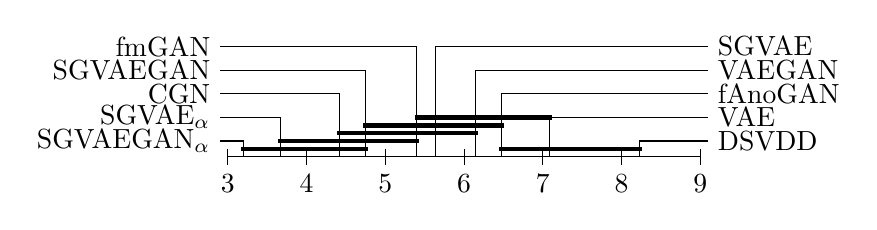
\begin{tikzpicture}[scale=1.0] 
  \draw (3.0,0) -- (9.0,0); 
  \foreach \x in {3,...,9} \draw (\x,0.10) -- (\x,-0.10) node[anchor=north]{$\x$}; 
  \draw (3.2,0) -- (3.2,0.19999999999999998) -- (2.9, 0.19999999999999998) node[anchor=east] {SGVAEGAN$_{\alpha}$}; 
  \draw (3.6625,0) -- (3.6625,0.5) -- (2.9, 0.5) node[anchor=east] {SGVAE$_{\alpha}$}; 
  \draw (4.4125,0) -- (4.4125,0.7999999999999999) -- (2.9, 0.7999999999999999) node[anchor=east] {CGN}; 
  \draw (4.75,0) -- (4.75,1.0999999999999999) -- (2.9, 1.0999999999999999) node[anchor=east] {SGVAEGAN}; 
  \draw (5.4,0) -- (5.4,1.4) -- (2.9, 1.4) node[anchor=east] {fmGAN}; 
  \draw (5.6375,0) -- (5.6375,1.4) -- (9.1, 1.4) node[anchor=west] {SGVAE}; 
  \draw (6.15,0) -- (6.15,1.0999999999999999) -- (9.1, 1.0999999999999999) node[anchor=west] {VAEGAN}; 
  \draw (6.475,0) -- (6.475,0.8) -- (9.1, 0.8) node[anchor=west] {fAnoGAN}; 
  \draw (7.0875,0) -- (7.0875,0.5) -- (9.1, 0.5) node[anchor=west] {VAE}; 
  \draw (8.225,0) -- (8.225,0.2) -- (9.1, 0.2) node[anchor=west] {DSVDD}; 
  \draw[line width=0.06cm,color=black,draw opacity=1.0] (3.170000047683716,0.1) -- (4.78,0.1); 
  \draw[line width=0.06cm,color=black,draw opacity=1.0] (3.6324999046325686,0.2) -- (5.430000095367432,0.2); 
  \draw[line width=0.06cm,color=black,draw opacity=1.0] (4.382499904632568,0.30000000000000004) -- (6.180000095367432,0.30000000000000004); 
  \draw[line width=0.06cm,color=black,draw opacity=1.0] (4.72,0.4) -- (6.504999904632569,0.4); 
  \draw[line width=0.06cm,color=black,draw opacity=1.0] (5.370000095367431,0.5) -- (7.117500095367432,0.5); 
  \draw[line width=0.06cm,color=black,draw opacity=1.0] (6.444999904632568,0.1) -- (8.255000381469726,0.1); 
 \end{tikzpicture} 
